\documentclass[11pt]{article}

% Packages
\usepackage[margin=1in]{geometry}
\usepackage{setspace}
\usepackage{titlesec}
\usepackage{graphicx}
\usepackage{booktabs}
\usepackage{amsmath}
\usepackage{hyperref}
\usepackage{float}
\usepackage{natbib}
\usepackage{subcaption}
\usepackage{threeparttable}
\usepackage{siunitx}
\usepackage{multirow}

\setstretch{1.15}

% Title formatting
\titleformat{\section}{\large\bfseries}{\thesection}{1em}{}
\titleformat{\subsection}{\normalsize\bfseries}{\thesubsection}{1em}{}

% Title info
\title{Airbnb NLP project}
\author{
Xianriu Cao \and Elvis Casco \and Rom\'{a}n Feria
}

\date{\today}

\begin{document}

\maketitle

\begin{abstract}
This project uses natural language processing to analyze Airbnb reviews in Barcelona and identify the factors that guests value most. The methodology combines TF--IDF, LDA topic modeling, and supervised classification. TF--IDF converts the review corpus into a weighted document-term matrix, LDA extracts four latent topics, and both Logistic Regression and Random Forest rank those topics by predictive importance. The dominant themes that emerge (host interaction, room quality, location and accessibility, and comfort and amenities, in that order) offer practical guidance for hosts and investors in Barcelona's short-term rental market.
\end{abstract}

\section{Introduction}

\subsection{Background}
Barcelona receives over 12 million international tourists per year, and Airbnb has become a significant part of its accommodation sector. For property owners and investors, understanding what drives a positive stay is directly relevant to competitive performance. Numerical ratings tell part of the story, but textual reviews give richer, more specific accounts of what visitors actually appreciated or disliked.

Several recent studies confirm the value of mining this text. \citet{safari2025sentiment} found that across six U.S.\ regions more than 90\% of Airbnb reviews are positive, and that review polarity matters more for host success than review volume. \citet{becerra2025reviews} showed that sentiment expressed in reviews has a stronger effect on listing prices than star ratings alone. \citet{perezsanchez2023sustainable} built a price prediction model that combines machine learning with sentiment scores derived from review text. These findings suggest that what guests write, not just how they rate, carries substantial information.

\subsection{Barcelona as a Case Study}
Barcelona is a well-studied case in this space. \citet{fernandezmorales2025mapping} applied text mining to Airbnb reviews across Mediterranean cities, including Barcelona, and confirmed the richness of the review content. On the regulatory side, Barcelona's PEUAT plan (2017) froze new short-term rental licenses in high-density zones \citep{ajuntament2017peuat}, though enforcement remains uneven and unlicensed listings persist \citep{seguillinares2019monitoring}. This regulatory pressure may itself shape the kinds of experiences that guests report.

Our data comes from Inside Airbnb \citep{cox2016airbnb}, an open-data initiative that scrapes and publishes listing and review information for cities worldwide.

\subsection{Research Question and Hypothesis}
The central question of this project is: which dimensions of the guest experience are most prominent in Barcelona's Airbnb reviews, and how do they rank in importance? We hypothesize that guest evaluations cluster around a small number of recurring themes and that interpersonal and experiential factors such as host interaction and room quality will outweigh supplementary aspects such as comfort and amenities.

\subsection{Motivation}
From a practical perspective, the results can help hosts prioritize the aspects of service that guests actually talk about, and help investors identify the property characteristics most likely to generate positive feedback. From a methodological perspective, the project demonstrates how TF--IDF, LDA, and supervised classification can be combined to systematically extract and rank thematic dimensions from a large corpus of unstructured text.

\section{Data}

\subsection{Source and Preparation}
The dataset was obtained from Inside Airbnb \citep{cox2016airbnb} and contains reviews from Barcelona. The raw dataset comprises 1,015,329 reviews with seven variables (listing ID, review ID, date, reviewer ID, reviewer name, original comment, and translated comment). Because reviews were originally written in Spanish, Catalan, French, English, and several other languages, all text was translated into English using Google Translate. After removing missing values and applying the preprocessing pipeline described in Section~\ref{sec:preproc}, the final corpus contains 100,172 reviews with one field: the cleaned review text.

\subsection{Exploratory Data Analysis}

Figure~\ref{fig:reviewlength} shows the distribution of review lengths. The majority of reviews are short: guests tend to express their evaluations concisely, focusing on the aspects they found most memorable. This brevity poses a challenge for LDA, which generally performs better on longer documents with richer context. To address this, we restricted the number of topics to a small, interpretable set.

\begin{figure}[H]
    \centering
    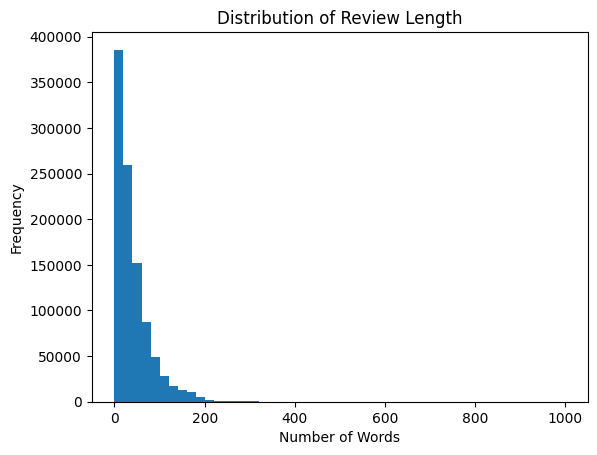
\includegraphics[width=0.7\textwidth]{figures/reviewlength.png}
    \caption{Distribution of review lengths in the corpus.}
    \label{fig:reviewlength}
\end{figure}

Figure~\ref{fig:wordfreq} shows the 20 most frequent terms in the corpus. ``Apartment'' leads with 517,852 occurrences, followed by ``great'' (417,583) and ``location'' (359,166). The total vocabulary contains 190,864 unique terms, but the distribution is highly skewed: the median frequency is 1, the mean is 106, and the 75th percentile is only 4. This long-tail pattern motivates the use of document-frequency thresholds in the TF--IDF step.

\begin{figure}[H]
    \centering
    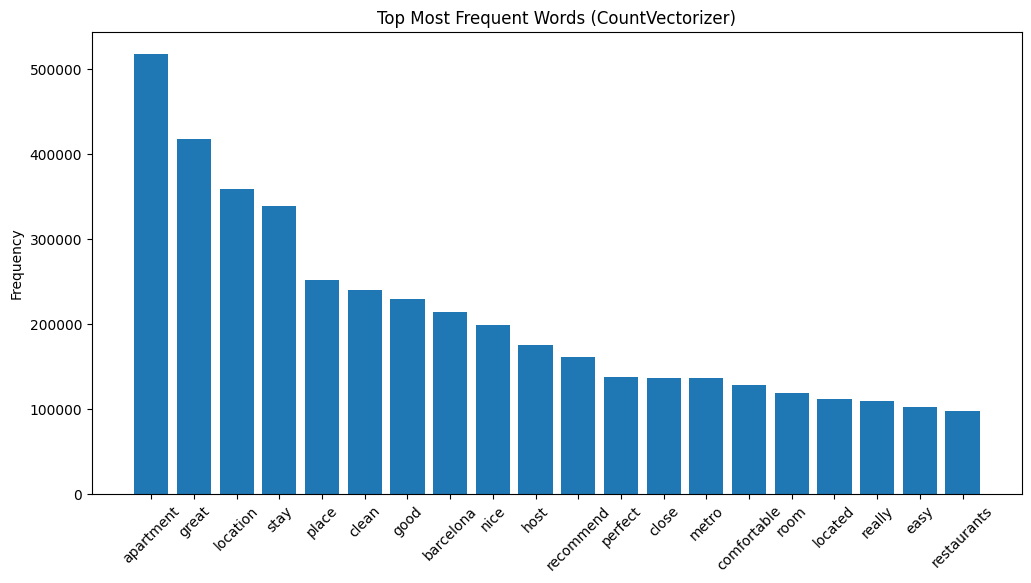
\includegraphics[width=0.7\textwidth]{figures/countvectorizer.png}
    \caption{Top 20 most frequent terms in the corpus. Counts are raw token occurrences across 100,172 reviews. Vocabulary size: 190,864 unique terms; median frequency: 1; mean: 106; max: 517,852.}
    \label{fig:wordfreq}
\end{figure}

\section{Methodology}

\subsection{Overview}
Our framework proceeds in four stages. First, the raw text is preprocessed and cleaned. Second, TF--IDF converts the cleaned corpus into a weighted document-term matrix. Third, LDA extracts four latent topics from the corpus. Fourth, Logistic Regression and Random Forest are trained on the TF--IDF features to predict review sentiment, and the resulting feature importances are combined with the LDA topic-word distributions to rank topics.

\subsection{Preprocessing}
\label{sec:preproc}
Standard text-cleaning steps were applied: lowercasing, punctuation and stopword removal, and lemmatization \citep{manning2008introduction}. The multilingual nature of the corpus required the additional translation step described above. Neural machine translation has reached a quality level where the noise introduced is generally acceptable for downstream NLP tasks, though it is not negligible and is discussed further in the limitations.

\subsection{TF--IDF}
TF--IDF (Term Frequency--Inverse Document Frequency) \citep{sparckjones1972statistical, ramos2003using} assigns each term a weight reflecting its frequency within a document relative to its frequency across the corpus. The IDF of a term $t$ is defined as:
\[
\mathrm{IDF}(t) = \log\!\left(\frac{N}{\mathrm{DF}(t)}\right) + 1,
\]
where $N$ is the total number of documents and $\mathrm{DF}(t)$ the number of documents containing $t$. The full weight is $\mathrm{TF\text{-}IDF}(t,d) = \mathrm{TF}(t,d) \times \mathrm{IDF}(t)$.

We included unigrams, bigrams, and trigrams in the vocabulary so that multi-word expressions like ``check in,'' ``public transport,'' and ``well equipped'' would be captured. We set \texttt{min\_df\,=\,200} and \texttt{max\_df\,=\,0.8}, guided by the term-frequency distribution. Table~\ref{tab:tfidf} shows the top terms by total TF--IDF weight across all reviews. Multi-word expressions such as ``stay family,'' ``access public,'' and ``central area'' receive the highest scores, since they are distinctive enough to appear in specific reviews but rare enough across the corpus to receive high IDF values.

\begin{table}[H]
\centering
\begin{threeparttable}
\caption{Top 10 terms by total TF--IDF weight.}
\label{tab:tfidf}
\begin{tabular}{@{}rlS[table-format=1.4]@{}}
\toprule
{Rank} & {Term} & {TF--IDF} \\
\midrule
1  & stay family      & 7.2113 \\
2  & access public    & 7.2113 \\
3  & destination      & 7.2113 \\
4  & central area     & 7.2064 \\
5  & stay clean       & 7.2064 \\
6  & apartment modern & 7.2064 \\
7  & good condition   & 7.2064 \\
8  & properly         & 7.2064 \\
9  & main street      & 7.2064 \\
10 & close shop       & 7.2064 \\
\bottomrule
\end{tabular}
\begin{tablenotes}\footnotesize
\item \textit{Notes:} TF--IDF scores are summed across all 100,172 documents. Vocabulary includes unigrams, bigrams, and trigrams with \texttt{min\_df\,=\,200} and \texttt{max\_df\,=\,0.8}.
\end{tablenotes}
\end{threeparttable}
\end{table}

\subsection{LDA Topic Modeling}
Latent Dirichlet Allocation \citep{blei2003latent} models each document as a mixture of topics, where each topic is a distribution over words. A key practical challenge is selecting the number of topics: coherence scores \citep{roder2015exploring} provide quantitative guidance, but the topics must also be interpretable.

Several studies have applied LDA to Airbnb reviews. \citet{jang2020determinants} extracted 43 topics from over a million New York City reviews. \citet{chong2020comparative} compared Hong Kong and Singapore and found 12 versus 5 topics, suggesting cross-cultural variation in what guests write about. \citet{luo2022visual} combined topic modeling with sentiment analysis for a visual recommendation system. Across these studies, the same broad themes recur: property and amenities, host and communication, location and accessibility, value for money.

We trained LDA models with $k = 3, 4, \ldots, 15$ topics and computed coherence scores for each (Figure~\ref{fig:coherence}). Scores ranged from 0.57 to 0.62 with no sharp peak, so we selected $k = 4$ as the configuration that produced the most interpretable groupings by human judgment.

\begin{figure}[H]
    \centering
    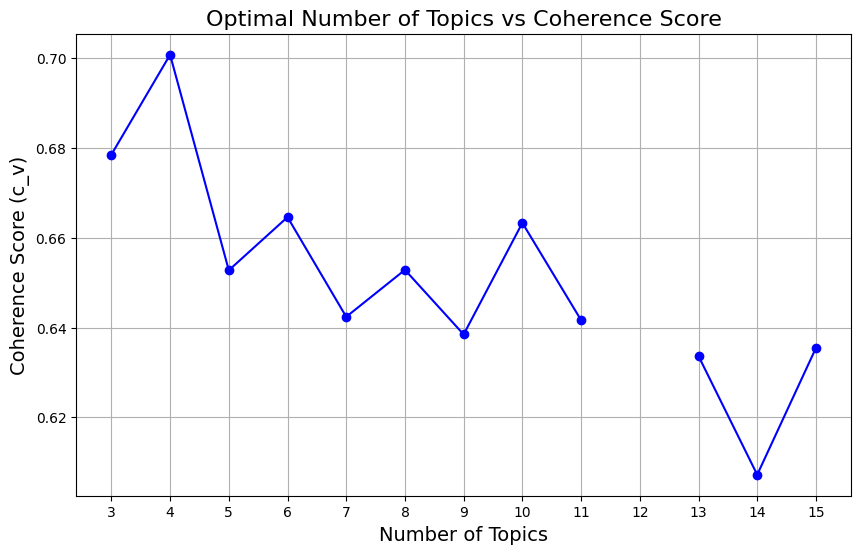
\includegraphics[width=0.7\textwidth]{figures/coherencescore.png}
    \caption{$C_v$ coherence score by number of topics ($k = 3$--$15$). Computed with Gensim; LDA trained with 2 passes per model. Custom stopwords removed (``apartment,'' ``stay,'' ``great,'' ``nice,'' ``good,'' ``place,'' ``location,'' ``barcelona''). Scores range from 0.57 to 0.62; $k = 4$ selected for interpretability.}
    \label{fig:coherence}
\end{figure}

Table~\ref{tab:lda} reports the four extracted topics with their top-10 words and associated weights. We assigned interpretive labels based on the word composition of each topic.

\begin{table}[H]
\centering
\begin{threeparttable}
\caption{LDA topics: top-10 words and weights ($k=4$).}
\label{tab:lda}
\small
\begin{tabular}{@{}clS[table-format=1.3]clS[table-format=1.3]@{}}
\toprule
\multicolumn{3}{c}{Topic 0: Comfort \& Amenities} & \multicolumn{3}{c}{Topic 1: Host Interaction} \\
\cmidrule(lr){1-3} \cmidrule(lr){4-6}
{} & {Word} & {Weight} & {} & {Word} & {Weight} \\
\midrule
1  & time        & 0.009 & 1  & recommend   & 0.028 \\
2  & comfortable & 0.009 & 2  & host        & 0.026 \\
3  & check       & 0.008 & 3  & clean       & 0.019 \\
4  & need        & 0.008 & 4  & perfect     & 0.018 \\
5  & day         & 0.007 & 5  & highly      & 0.012 \\
6  & clean       & 0.007 & 6  & close       & 0.011 \\
7  & bed         & 0.006 & 7  & need        & 0.011 \\
8  & helpful     & 0.006 & 8  & definitely  & 0.010 \\
9  & space       & 0.006 & 9  & easy        & 0.010 \\
10 & kitchen     & 0.006 & 10 & thank       & 0.010 \\
\midrule
\multicolumn{3}{c}{Topic 2: Location \& Accessibility} & \multicolumn{3}{c}{Topic 3: Room Quality} \\
\cmidrule(lr){1-3} \cmidrule(lr){4-6}
{} & {Word} & {Weight} & {} & {Word} & {Weight} \\
\midrule
1  & metro      & 0.023 & 1  & room      & 0.017 \\
2  & walk       & 0.018 & 2  & clean     & 0.014 \\
3  & minute     & 0.016 & 3  & host      & 0.014 \\
4  & close      & 0.015 & 4  & excellent & 0.010 \\
5  & area       & 0.012 & 5  & bed       & 0.008 \\
6  & clean      & 0.012 & 6  & thank     & 0.008 \\
7  & restaurant & 0.011 & 7  & bathroom  & 0.008 \\
8  & locate     & 0.010 & 8  & locate    & 0.007 \\
9  & station    & 0.010 & 9  & kitchen   & 0.007 \\
10 & away       & 0.009 & 10 & small     & 0.007 \\
\bottomrule
\end{tabular}
\begin{tablenotes}\footnotesize
\item \textit{Notes:} Weights are word-topic probabilities from LDA trained with \texttt{LdaMulticore} (4 topics, 10 passes). Topic labels assigned by the authors based on word composition.
\end{tablenotes}
\end{threeparttable}
\end{table}

Topic 0 groups words related to practical aspects of the stay such as beds, kitchen, and available space. Topic 1 centers on the host and recommendation language, suggesting that host quality is closely tied to whether guests recommend the listing. Topic 2 captures proximity to transport and local amenities. Topic 3 focuses on the physical room and its condition. Word clouds for each topic are shown in Figure~\ref{fig:wordclouds}. Topic distributions were validated: all 100,172 documents have topic shares that sum to one.

\begin{figure}[H]
    \centering
    \begin{subfigure}[b]{0.45\textwidth}
        \centering
        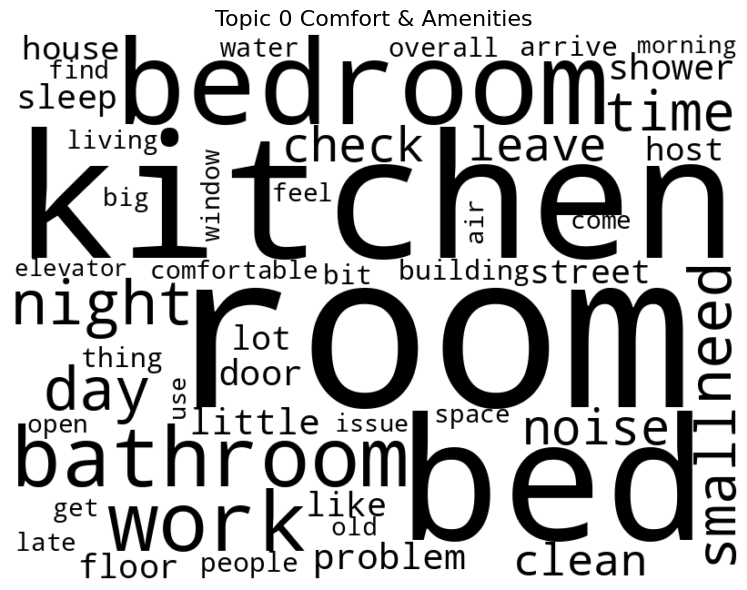
\includegraphics[width=\textwidth]{figures/topic0.png}
        \caption{Topic 0: Comfort \& Amenities}
    \end{subfigure}
    \hfill
    \begin{subfigure}[b]{0.45\textwidth}
        \centering
        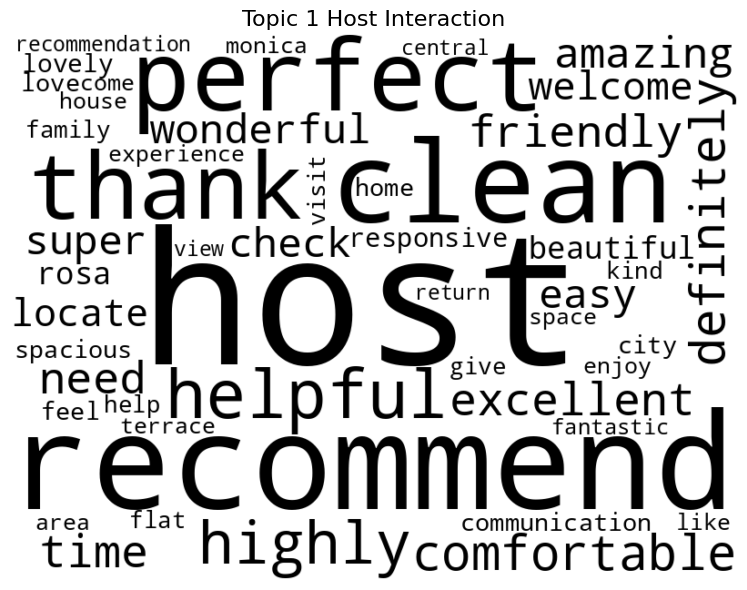
\includegraphics[width=\textwidth]{figures/topic1.png}
        \caption{Topic 1: Host Interaction}
    \end{subfigure}\\[0.5em]
    \begin{subfigure}[b]{0.45\textwidth}
        \centering
        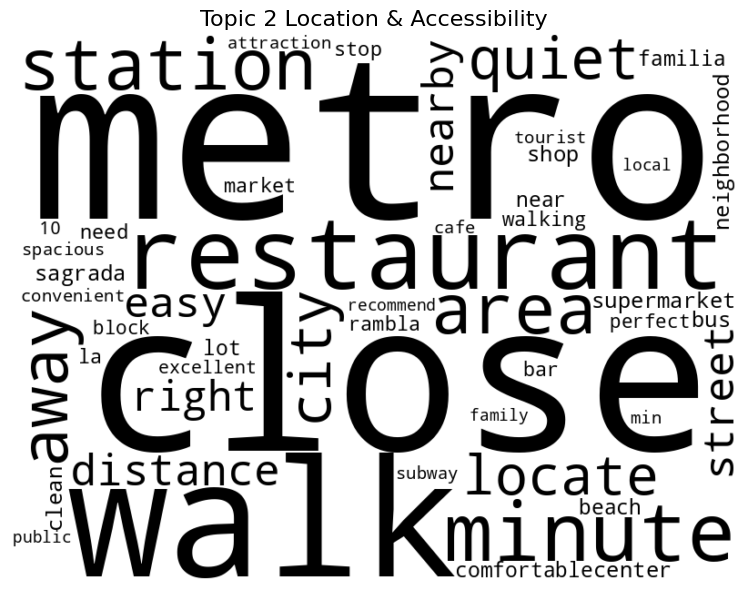
\includegraphics[width=\textwidth]{figures/topic2.png}
        \caption{Topic 2: Location \& Accessibility}
    \end{subfigure}
    \hfill
    \begin{subfigure}[b]{0.45\textwidth}
        \centering
        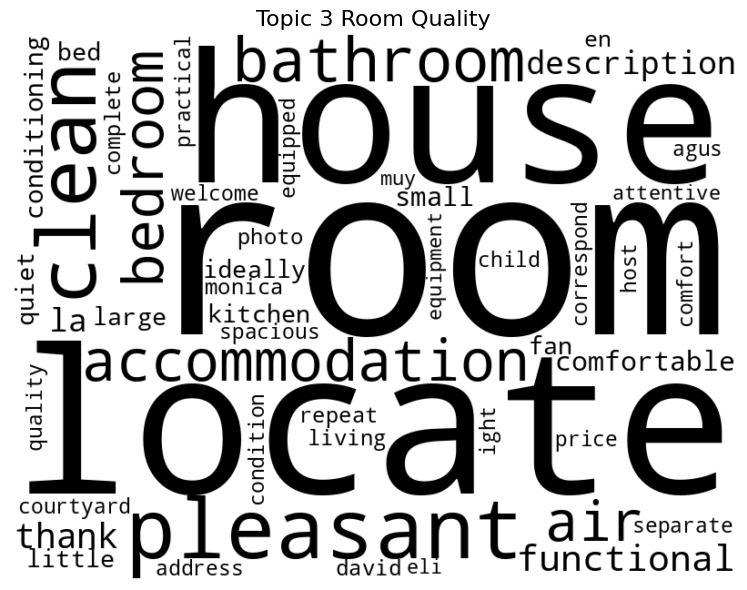
\includegraphics[width=\textwidth]{figures/topic3.png}
        \caption{Topic 3: Room Quality}
    \end{subfigure}
    \caption{Word clouds for the four LDA topics.}
    \label{fig:wordclouds}
\end{figure}

These four topics align with the recurring dimensions identified in the literature: property and amenities, host and communication, location and accessibility, and value for money \citep{jang2020determinants, chong2020comparative}. The supervised classification step described next uses these topic distributions, together with the TF--IDF features, to determine which of the four topics is most strongly associated with review sentiment.

\subsection{Sentiment Analysis and Label Generation}
Since the dataset does not include explicit sentiment labels, we generated a binary target variable using TextBlob \citep{loria2020textblob}. Each review was assigned a polarity score, and reviews with positive polarity were labeled 1 (positive) and the rest 0 (negative).

A well-known issue in this domain is positivity bias: the vast majority of Airbnb reviews are positive, creating severe class imbalance. This is handled through class weighting in the supervised step \citep{he2009learning}.

Cross-platform work by \citet{kaya2024analysing} comparing Booking.com and Expedia confirms that sentiment patterns are partly platform-specific, which motivates analyzing Airbnb reviews on their own terms. Within the Airbnb literature, \citet{santos2022expressing} identified themes driving satisfaction and dissatisfaction in Fortaleza, Brazil, and \citet{agarwal2024investigating} combined NLP with Random Forest and GIS to segment listings by review-based sentiment.

\subsection{Supervised Classification}
We trained both Logistic Regression and Random Forest on the TF--IDF features to predict the sentiment labels.

Logistic Regression \citep{pang2002thumbs, jurafsky2023speech} was chosen for its interpretability: its coefficients indicate directly which terms are associated with each class. Random Forest \citep{breiman2001random} can capture non-linear feature interactions and provides built-in feature importance scores. Both models used \texttt{class\_weight="balanced"} to account for the class imbalance \citep{he2009learning}. The data was split 80/20 into training and test sets with a fixed random seed.

To rank the LDA topics, we computed a weighted average of each model's feature-level scores (coefficients for Logistic Regression, importances for Random Forest) using the top 15 words of each LDA topic as weights. The resulting per-topic scores were normalized to a 0--1 scale using min-max scaling and averaged across the two models.

%% ============================================================
\section{Results}
%% ============================================================

\subsection{Sentiment Label Distribution}
Out of 100,172 reviews, 86,222 (86.1\%) were labeled as positive and 13,950 (13.9\%) as negative (Figure~\ref{fig:sentiment}). This confirms the strong positivity bias reported in the literature and justifies the use of balanced class weights.

\begin{figure}[H]
    \centering
    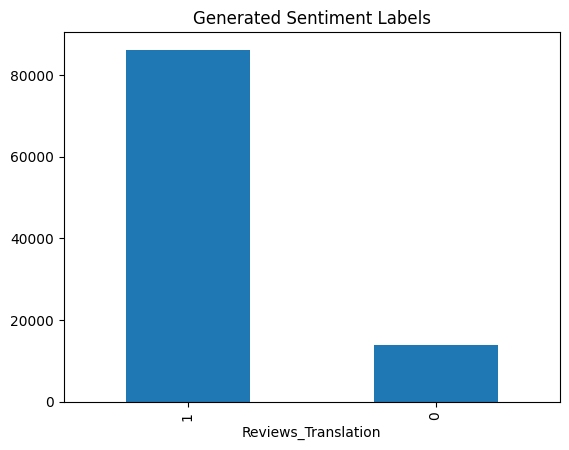
\includegraphics[width=0.55\textwidth]{figures/sentiment_labels.png}
    \caption{Distribution of sentiment labels.}
    \label{fig:sentiment}
\end{figure}

\subsection{Classification Performance}

\subsubsection{Logistic Regression}

Table~\ref{tab:logreg} reports the classification results for Logistic Regression. The model achieves 95\% accuracy and a ROC-AUC of 0.99. It detects negative reviews with high recall (0.97) but lower precision (0.76), meaning it flags most negative reviews at the cost of some false positives.

\begin{table}[H]
\centering
\begin{threeparttable}
\caption{Logistic Regression: classification report and confusion matrix.}
\label{tab:logreg}
\begin{tabular}{@{}lS[table-format=1.2]S[table-format=1.2]S[table-format=1.2]r@{}}
\toprule
{Class} & {Precision} & {Recall} & {F1-score} & {Support} \\
\midrule
Negative (0) & 0.76 & 0.97 & 0.85 &  2,740 \\
Positive (1) & 0.99 & 0.95 & 0.97 & 17,295 \\
\midrule
Macro avg    & 0.88 & 0.96 & 0.91 & 20,035 \\
Weighted avg & 0.96 & 0.95 & 0.96 & 20,035 \\
\midrule
\multicolumn{5}{@{}l}{Accuracy: 0.95 \quad ROC-AUC: 0.992} \\
\bottomrule
\end{tabular}
\begin{tablenotes}\footnotesize
\item[]
\begin{tabular}{@{}lrr@{}}
& Predicted 0 & Predicted 1 \\
Actual 0 & 2,645 &    95 \\
Actual 1 &   813 & 16,482 \\
\end{tabular}
\item \textit{Notes:} \texttt{class\_weight="balanced"}, \texttt{max\_iter=1000}. Train/test split: 80/20, \texttt{random\_state=42}.
\end{tablenotes}
\end{threeparttable}
\end{table}

Figure~\ref{fig:posneg} shows the strongest positive and negative coefficients. The top positive terms (``great'' at 17.18, ``good'' at 15.64, ``nice'' at 13.69) are general satisfaction words, while the top negative terms (``bad'' at $-6.73$, ``dirty'' at $-5.59$, ``unfortunately'' at $-4.29$) point to specific complaints about cleanliness, comfort, and unmet expectations.

\begin{figure}[H]
    \centering
    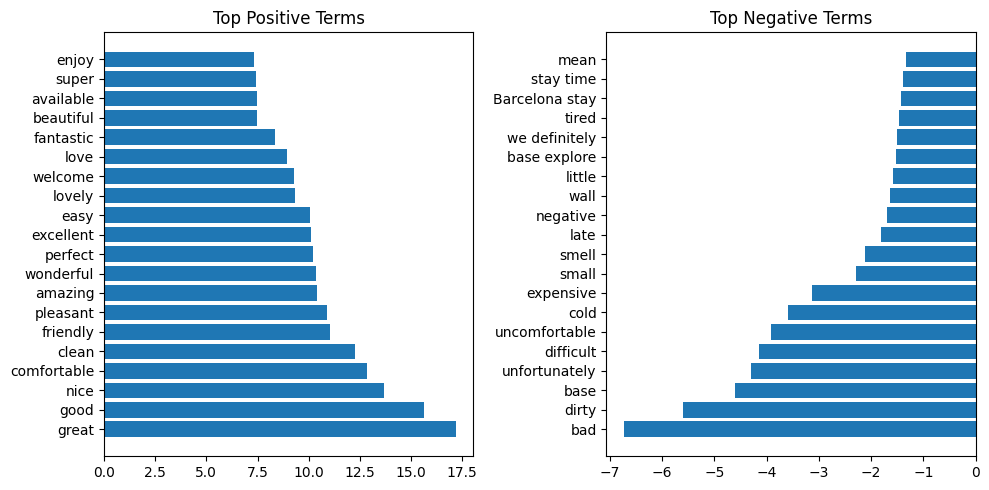
\includegraphics[width=0.75\textwidth]{figures/positive_negative.png}
    \caption{Top positive and negative terms from Logistic Regression coefficients. Larger positive (negative) values indicate stronger association with the positive (negative) class.}
    \label{fig:posneg}
\end{figure}

\subsubsection{Random Forest}

Table~\ref{tab:rf} reports the classification results for Random Forest. The model achieves 97\% accuracy and a ROC-AUC of 0.99. Compared with Logistic Regression, it has higher precision on the negative class (0.94 vs.\ 0.76) but lower recall (0.84 vs.\ 0.97).

\begin{table}[H]
\centering
\begin{threeparttable}
\caption{Random Forest: classification report and confusion matrix.}
\label{tab:rf}
\begin{tabular}{@{}lS[table-format=1.2]S[table-format=1.2]S[table-format=1.2]r@{}}
\toprule
{Class} & {Precision} & {Recall} & {F1-score} & {Support} \\
\midrule
Negative (0) & 0.94 & 0.84 & 0.89 &  2,740 \\
Positive (1) & 0.97 & 0.99 & 0.98 & 17,295 \\
\midrule
Macro avg    & 0.96 & 0.91 & 0.93 & 20,035 \\
Weighted avg & 0.97 & 0.97 & 0.97 & 20,035 \\
\midrule
\multicolumn{5}{@{}l}{Accuracy: 0.97 \quad ROC-AUC: 0.988} \\
\bottomrule
\end{tabular}
\begin{tablenotes}\footnotesize
\item[]
\begin{tabular}{@{}lrr@{}}
& Predicted 0 & Predicted 1 \\
Actual 0 & 2,291 &   449 \\
Actual 1 &   142 & 17,153 \\
\end{tabular}
\item \textit{Notes:} \texttt{n\_estimators=200}, \texttt{class\_weight="balanced"}, \texttt{random\_state=42}. Same train/test split as Logistic Regression.
\end{tablenotes}
\end{threeparttable}
\end{table}

Figure~\ref{fig:rftop} shows the top terms by Random Forest feature importance (mean decrease in Gini impurity across 200 trees). Unlike Logistic Regression, these importances are non-negative and do not distinguish between positive and negative associations. The ranking is led by ``great'' (0.073), ``good'' (0.048), ``location'' (0.044), and ``apartment'' (0.041), with ``host'' appearing at rank 10 (0.020).

\begin{figure}[H]
    \centering
    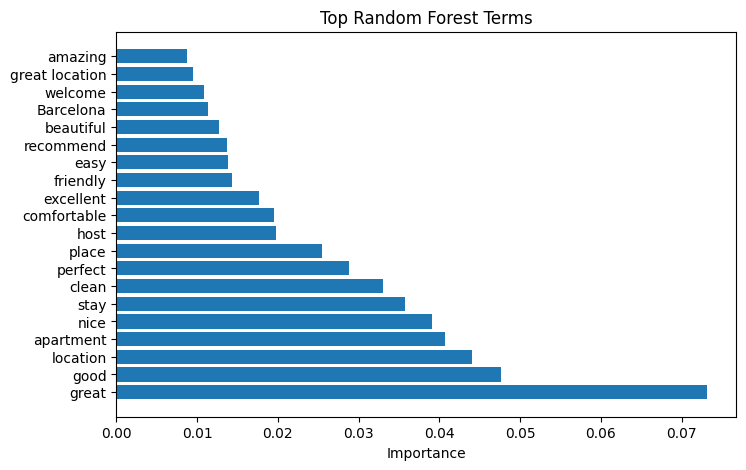
\includegraphics[width=0.7\textwidth]{figures/top_random_forest_terms.png}
    \caption{Top 20 terms by Random Forest feature importance. Values represent mean decrease in Gini impurity, averaged across 200 trees.}
    \label{fig:rftop}
\end{figure}

\subsubsection{Model Comparison}

Figure~\ref{fig:roc} overlays the ROC curves of both models. Both achieve near-identical AUC values, but they differ in the precision-recall trade-off on the minority class: Logistic Regression prioritizes recall (catching negatives), while Random Forest prioritizes precision (avoiding false alarms).

\begin{figure}[H]
    \centering
    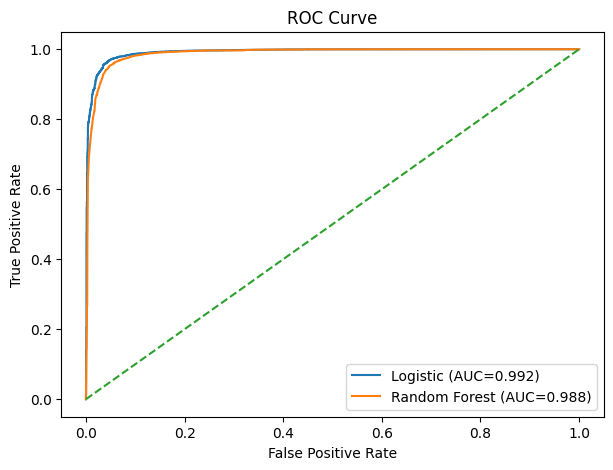
\includegraphics[width=0.55\textwidth]{figures/roc_curve.png}
    \caption{ROC curves: Logistic Regression vs.\ Random Forest.}
    \label{fig:roc}
\end{figure}

\subsection{Topic Importance}
Table~\ref{tab:importance} combines the per-topic scores from both models. The raw scores differ in scale (Logistic Regression coefficients vs.\ Random Forest impurity reductions), so each column was normalized to $[0, 1]$ before averaging.

\begin{table}[H]
\centering
\begin{threeparttable}
\caption{Topic importance: raw scores, normalized scores, and combined ranking.}
\label{tab:importance}
\begin{tabular}{@{}clS[table-format=1.3]S[table-format=1.4]S[table-format=1.3]S[table-format=1.3]S[table-format=1.3]@{}}
\toprule
{Topic} & {Label} & {Log.\ Reg.} & {Rand.\ Forest} & {Log.\ (norm.)} & {RF (norm.)} & {Average} \\
\midrule
1 & Host Interaction          & 4.305 & 0.0144 & 1.000 & 1.000 & 1.000 \\
3 & Room Quality              & 3.085 & 0.0095 & 0.211 & 0.323 & 0.267 \\
2 & Location \& Access.       & 2.790 & 0.0072 & 0.020 & 0.007 & 0.014 \\
0 & Comfort \& Amenities      & 2.759 & 0.0072 & 0.000 & 0.000 & 0.000 \\
\bottomrule
\end{tabular}
\begin{tablenotes}\footnotesize
\item \textit{Notes:} Raw scores are weighted averages of model feature scores using LDA topic-word probabilities (top 15 words per topic). Normalization: min-max scaling per column. Average: arithmetic mean of normalized Logistic Regression and Random Forest scores.
\end{tablenotes}
\end{threeparttable}
\end{table}

\begin{figure}[H]
    \centering
    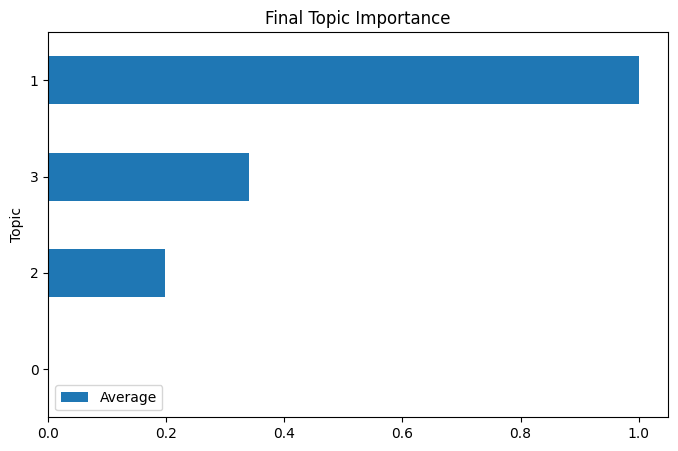
\includegraphics[width=0.6\textwidth]{figures/final_topic_importance.png}
    \caption{Combined normalized topic importance.}
    \label{fig:importance}
\end{figure}

Host Interaction (Topic 1) is by far the most important dimension, with a normalized score of 1.000 in both models. Room Quality (Topic 3) follows at a considerable distance (0.267). Location \& Accessibility (Topic 2) and Comfort \& Amenities (Topic 0) contribute very little (0.014 and 0.000 respectively). This ranking is consistent across both classifiers, which strengthens the finding. The result also aligns with the literature: \citet{jang2020determinants} and \citet{chong2020comparative} similarly found host-related topics among the most prominent dimensions in Airbnb reviews.

\section{Conclusion}

This project applied TF--IDF, LDA topic modeling, and supervised classification to over 100,000 Airbnb reviews from Barcelona. Guest reviews cluster around four themes: host interaction, room quality, location and accessibility, and comfort and amenities.

The key finding is that host interaction stands out as the dominant factor associated with review sentiment, followed by room quality. Location and comfort, while frequently mentioned, contribute relatively little to distinguishing positive from negative experiences. This suggests that the interpersonal dimension of the stay, how the host communicates and responds to needs, plays a larger role in shaping satisfaction than physical or locational attributes.

These results have practical implications. Hosts looking to improve their reviews should prioritize responsiveness and personal attention. Investors evaluating properties for short-term rental should consider not only location and amenities but also the feasibility of delivering a high-quality hosting experience.

\section{Limitations}

Several limitations should be noted. First, the translation of reviews from multiple languages into English through neural machine translation inevitably introduces noise. Modern tools perform well in general, but they may miss nuances, idiomatic expressions, or culturally specific references that could affect the analysis.

Second, the sentiment labels were generated automatically using TextBlob \citep{loria2020textblob} rather than through manual annotation. The labels therefore reflect the model's assessment of polarity, which may not always align with human interpretation. The severe class imbalance (86\% positive) also limits the classifiers' ability to learn from negative reviews.

Third, LDA assumes that each document is a mixture of topics, but many Airbnb reviews are only a few sentences long, which limits the contextual information available for topic assignment. This may produce noisier topic distributions for individual reviews, even though the aggregate patterns remain interpretable.

Fourth, the analysis is cross-sectional and descriptive. The models identify associations between textual features and sentiment, but they do not establish causal relationships. We cannot conclude that improving host communication will cause better reviews, only that positive reviews tend to emphasize host interaction more strongly.

Finally, the dataset covers only Barcelona, and the findings may not generalize to other cities with different tourism profiles, regulatory environments, or guest expectations.

\bibliographystyle{apalike}
\bibliography{references}

\end{document}
